%%%%%%%%%%%%%%%%%%
% Document class %
%%%%%%%%%%%%%%%%%%

\documentclass[a4paper, 12pt]{article}


%%%%%%%%%%%%
% Packages %
%%%%%%%%%%%%

\usepackage[english]{babel}
\usepackage[noheader]{packages/sleek}
\usepackage{packages/sleek-title}


%%%%%%%%%%%%%%%%%%%%
% Title page setup %
%%%%%%%%%%%%%%%%%%%%

\logo{resources/pdf/logo-uliege.pdf}
\institute{University of Liège}
\faculty{Faculty of Applied Science}
\title{Securing network with firewalls and\\NATs}
\subtitle{Step 1: drawing the network}
\author{Maxime \textsc{Meurisse}\\Valentin \textsc{Vermeylen}}
\context{Master in Civil Engineering}
\date{Academic year 2020-2021}


%%%%%%%%%%%%
% Document %
%%%%%%%%%%%%

\begin{document}
	\maketitle
	
	\section{Drawing of the network}
	
	The representation of the network topology is shown in Figure \ref{fig:network.topology}. This figure is in vector format: it is possible to zoom in on it for better reading without loss of quality.
	
	\begin{figure}[H]
	    \centering
	    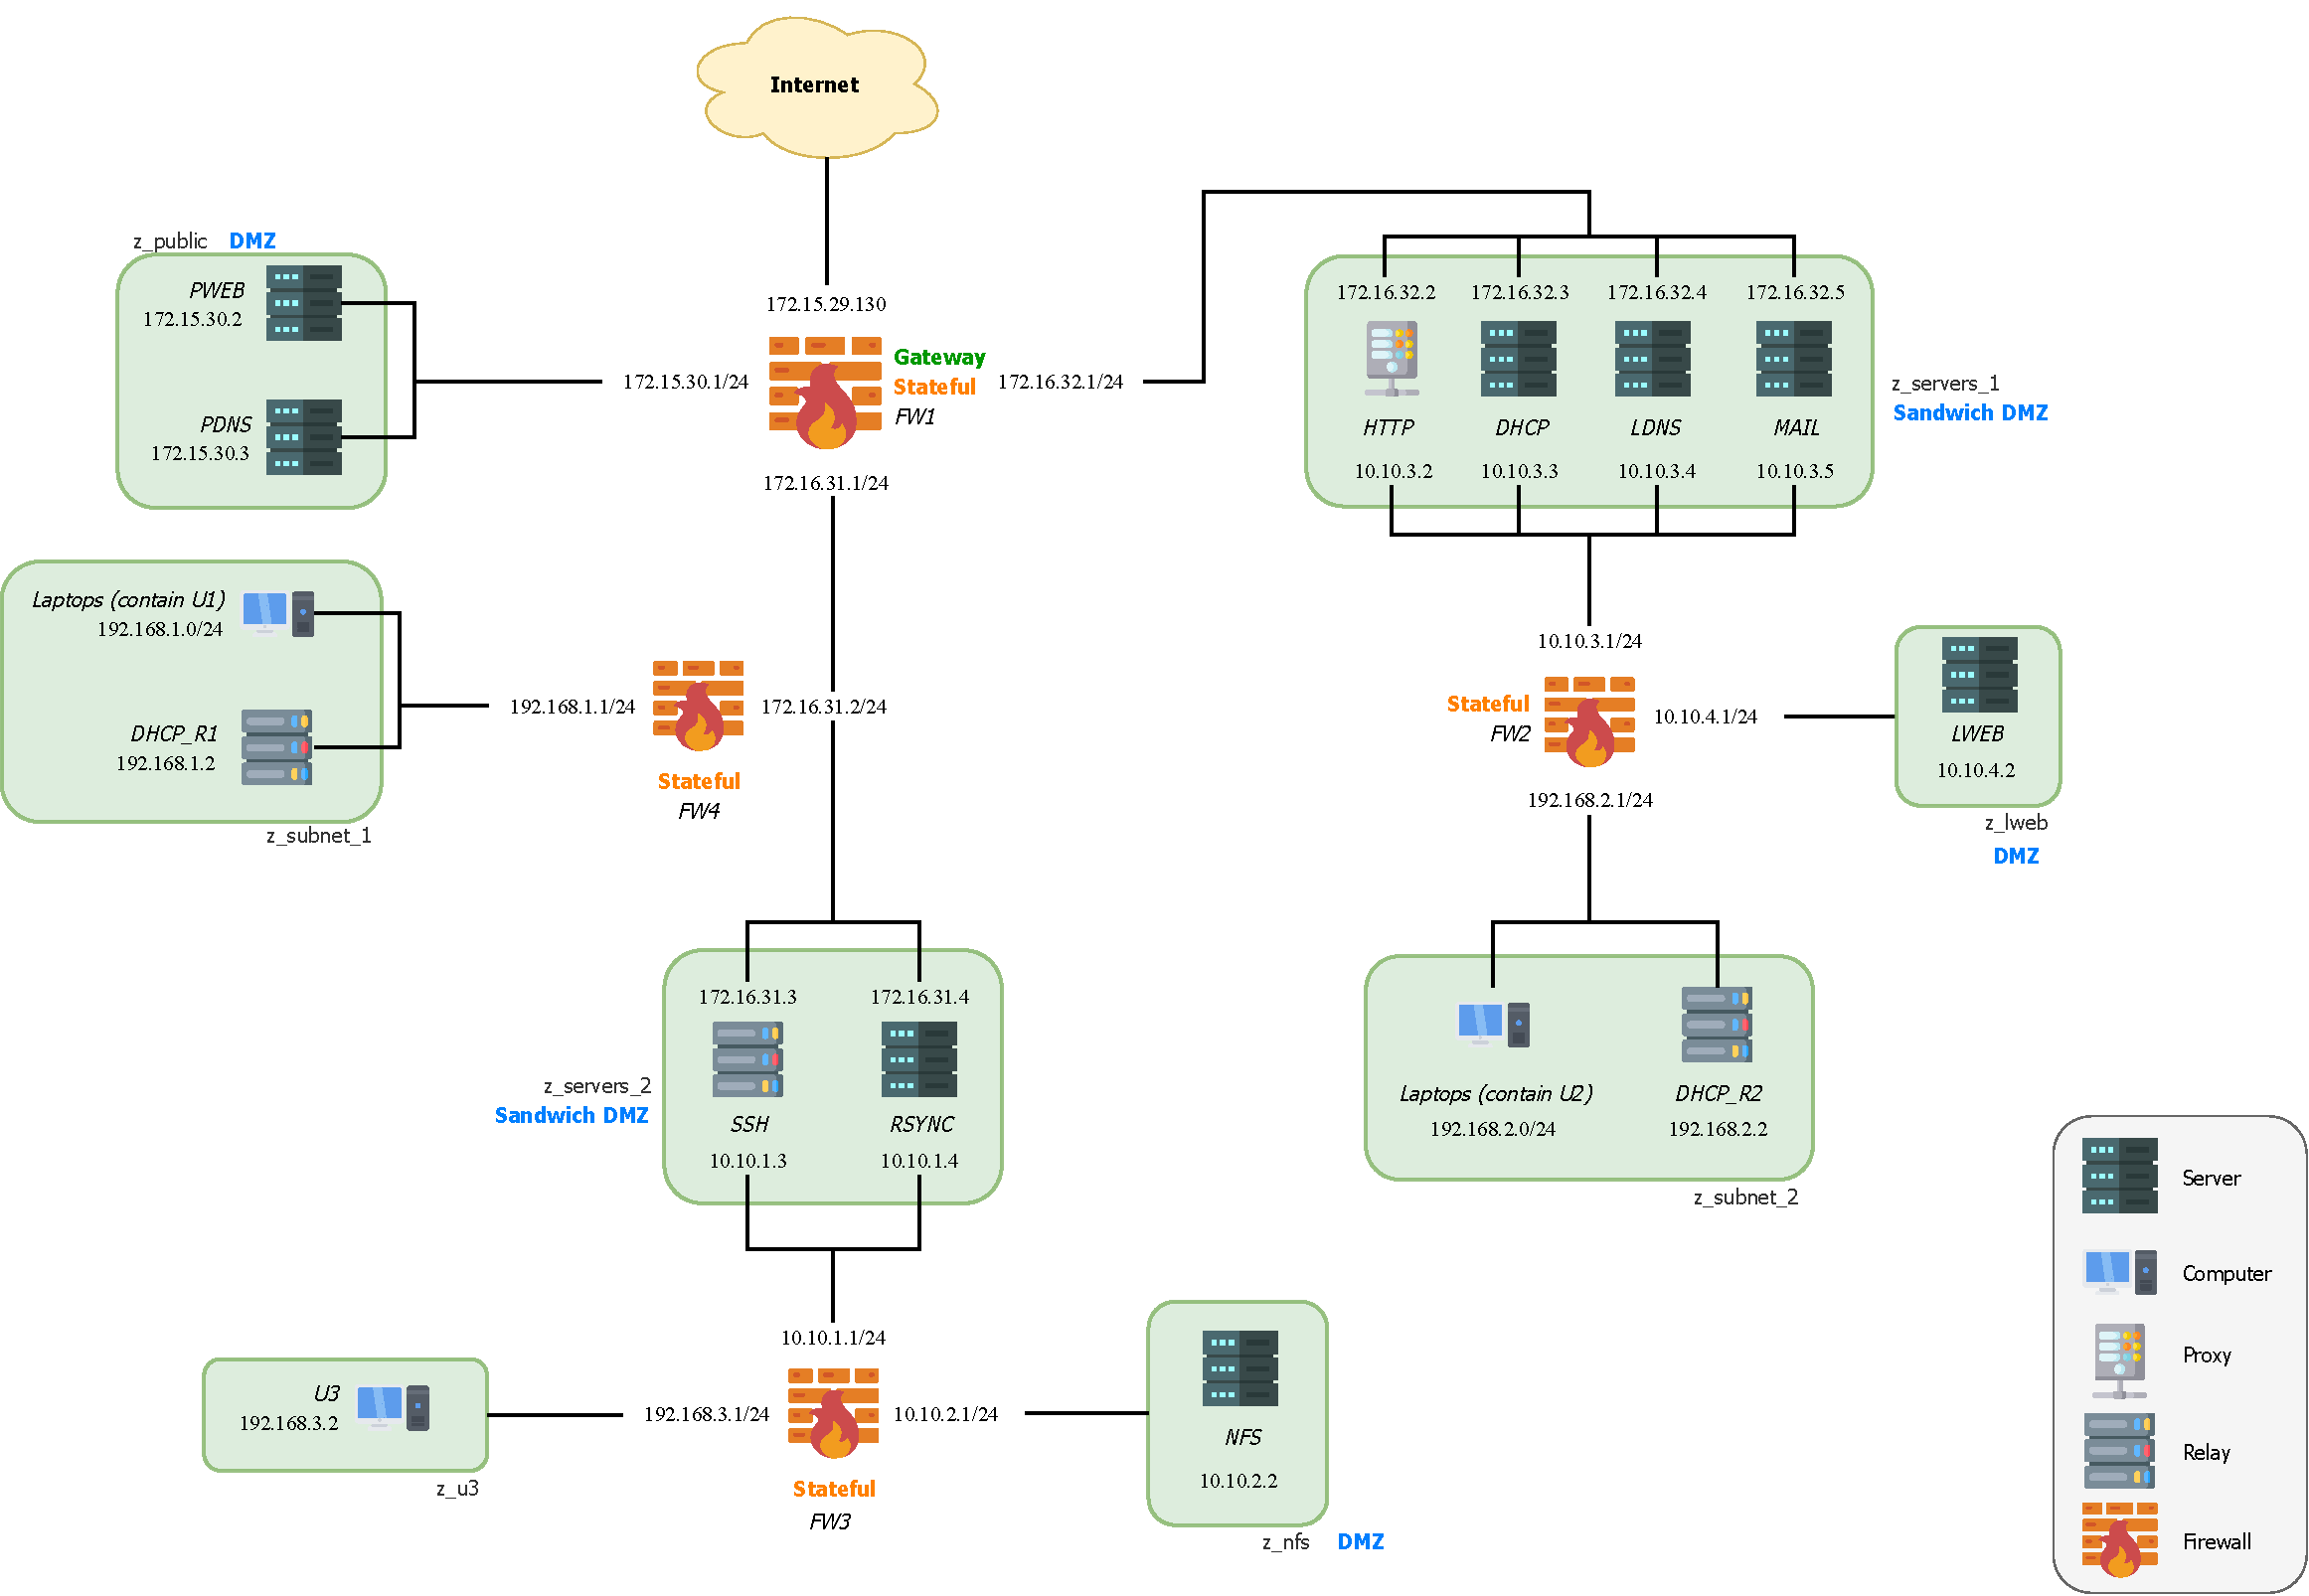
\includegraphics[width=0.9\textwidth]{resources/pdf/topology.pdf}
	    \caption{Topology of the network.}
	    \label{fig:network.topology}
	\end{figure}
	
	\section{Details of the network}
	
	This network is composed of 4 firewalls, 8 zones and several types of devices (servers, proxies, computers and relays).
	
	\subsection{Firewalls}
	
	The 4 firewalls present in the network are \emph{stateful} firewalls.
	
	The firewall \emph{FW1} is a gateway: it acts as a link between the Internet and the company's internal network. A NAT configuration will be necessary on this firewall (on interface \texttt{172.15.29.130}).
	
	The other firewalls (\emph{FW2}, \emph{FW3} and \emph{FW4}) are \enquote{classical} firewalls that do not act as NATs.
	
	\subsection{Zones}
	
	The network is composed of 8 zones: \emph{z\_public}, \emph{z\_servers\_1}, \emph{z\_servers\_2}, \emph{z\_lweb}, \emph{z\_subnet\_1}, \emph{z\_subnet\_2}, \emph{z\_u3} and \emph{z\_nfs}. Each zone has been defined by grouping together devices that have the same IP address prefix.
	
	The \emph{z\_public}, \emph{z\_lweb} and \emph{z\_nfs} zones are \emph{DMZ}. The \emph{z\_servers\_1} and \emph{z\_servers\_2} zones are \emph{sandwich DMZ} (because zones are between 2 firewalls). These zones are considered as DMZ because they are connected neither to the Internet, or the internal network. The internal network is represented by \emph{z\_subnet\_1}, \emph{z\_subnet\_2} and \emph{z\_u3} zones (each zone composed of devices with \texttt{192.168.X.X} as private IP address prefix).
	
	\subsubsection{Zone classification}
	
	For each firewall, zones are classified from more secured to less secured. We decided for the zones containing the laptops to be the most secure ones (the ones requiring the most security) because humans are usually the least reliable part of a system, more so if the laptops come from an external environment to the company. We initially only considered a zone to one firewall (the least deep one), as we believed it to be done in the exercise session. However, it is probably more correct to consider one zone in every firewall it is linked to, and that is done in the NB below. All justifications given after stay the same, but more are added in the NB if there are more zones to be considered for the given firewall. In the first part, FW4 thus only has one zone (\emph{z\_subnet\_1}), but it has 2 zones in the NB.
	
	Since we need to take care of every interface in the rules of a firewall, the NB is probably more correct, but we still kept the below hierarchies too since we are not totally certain which one is expected.
	
	\begin{itemize}
	    \item \emph{FW1}
	    \begin{itemize}
	        \item \emph{z\_servers\_2}
	        \item \emph{z\_servers\_1}
	        \item \emph{z\_public}
	    \end{itemize}
    \end{itemize}
    
    For this firewall, we have considered that \emph{z\_servers\_1} requires more security than \emph{z\_public} because the servers in zone \emph{z\_servers\_1} are used within the internal company network and certainly manage sensitive data (confidential emails, etc). The servers in zone \emph{z\_public} are public and certainly contain less sensitive or private information of the company. We therefore believe the four other servers require more security, since they are meant to be only used internally. And we consider \emph{z\_servers\_2} to require more security than \emph{z\_servers\_1} since it contains RSYNC, which serves as backup for the laptops in the network and must thus be more protected in our opinion (and the ssh relay is used to connect to the Internet).
    
    \begin{itemize}
	    \item \emph{FW2}
	    \begin{itemize}
	        \item \emph{z\_subnet\_2}
	        \item \emph{z\_lweb}
	    \end{itemize}
    \end{itemize}
    
    For this firewall, we have considered that \emph{z\_subnet\_2} requires more security than \emph{z\_lweb} because zone \emph{z\_subnet\_2} contains all the employees' computers connected to the company's internal network. These computers can contain anything, therefore potentially malware aimed at attacking the company, and so their internal traffic must be carefully controlled, as well as their external traffic to avoid getting malwares inadvertently. These computers can also contain sensitive (and private) data. The private web server is only used internally by the laptops, and so requires less security (and it cannot be accessed by the Internet, only by the laptops in the subnets for communicating internal information that do not seem, to us, to require a lot of security, \textit{i.e.} schedules, news,...), so it ranks lower on the above hierarchy. 
    
    \begin{itemize}
	    \item \emph{FW3}
	    \begin{itemize}
	        \item \emph{z\_u3}
	        \item \emph{z\_nfs}
	    \end{itemize}
    \end{itemize}
    
    For this firewall, we have considered that \emph{z\_u3} requires more security than \emph{z\_nfs} because the NFS server is only used by U3 to store documents (although other clients may access it theoretically). Furthermore, U3 can access the Internet and other devices in the network via ssh (and may contain private and sensitive data), and so requires more security. 
    
    \begin{itemize}
	    \item \emph{FW4}
	    \begin{itemize}
	        \item \emph{z\_subnet\_1}
	    \end{itemize}
	\end{itemize}
	
	\textbf{NB} : We only considered a zone to be associated to one firewall, but if we wanted to have, per firewall, all zones attached to it in a hierarchy, the above justifications stay the same, but we could have on top of them the following ones (FW1 stays the same and is thus not reported) : 
    
    \begin{itemize}
	    \item \emph{FW2}
	    \begin{itemize}
	        \item \emph{z\_subnet\_2}
	        \item \emph{z\_servers\_1}
	        \item \emph{z\_lweb}
	    \end{itemize}
    \end{itemize}
    
    For reasons exposed before for the web server, and because the server\_1 is accessed by the laptops in subnet\_2, and so that accessing subnet needs therefore to be more secured. We decided to have the zone containing the laptops as the one requiring the most security.
    
    \begin{itemize}
	    \item \emph{FW3}
	    \begin{itemize}
	        \item \emph{z\_u3}
	        \item \emph{z\_servers\_2}
	        \item \emph{z\_nfs}
	    \end{itemize}
    \end{itemize}
    
    Because U3 is not secured anywhere else, and can access the Internet via ssh in the servers\_2 (and same justification for nfs placement as before). U3 is also a computer used by a human, so we want it to be more secured. servers\_2 contains the RSYNC server, which is used by the laptops in the private networks to backup documents, and so we considered it more secured than the NFS, which is only used by U3 for backup.
    
    \begin{itemize}
	    \item \emph{FW4}
	    \begin{itemize}
	        \item \emph{z\_subnet\_1}
	        \item \emph{z\_servers\_2}
	    \end{itemize}
	\end{itemize}
	
	For this firewall, we have considered that \emph{z\_subnet\_1} is more secured than \emph{z\_servers\_2} because zone \emph{z\_subnet\_1}, like zone \emph{z\_subnet\_2}, contains all the employees' computers connected to the company's internal network. These computers can contain anything, therefore potentially malware aimed at attacking the company, and so their internal traffic must be carefully controlled, as well as their external traffic to avoid getting malwares inadvertently. These computers can also contain sensitive (and private) data. Moreover, the RSYNC server is only accessible by the internal computers of the network mentioned above, so those computers require more security to ensure that of RSYNC. The same is true for the SSH server, it is accessed by the laptops (and is only a relay, so it requires less security).
	
	\subsection{Devices}
	
	The network is composed of several devices. The type of each device is represented by its icon (explained in the representation's legend). Note that in zones \emph{z\_subnet\_1} and \emph{z\_subnet\_2}, company computers (\enquote{Laptops}) cannot have the same IP address as the DHCP relay in the same zone or the firewall interface and do not have a static IP address. They have dynamic IP addresses determined by the DHCP server (through DHCP relays).
\end{document} 
